\documentclass{standalone}
\usepackage{tikz}

\begin{document}

\begin{minipage}{0.55\textwidth}
	\centering
	\def\rowperm{{0, 1, 2, 3, 4, 5, 6}}
	%\def\colperm{{0, 1, 2, 3, 4, 5, 6}}
	\def\colperm{{0, 1, 2, 3, 4, 5, 6}}
	\scalebox{0.7}{\begin{tikzpicture}
		\foreach \x in {0,1}
		\fill[gray] (\colperm[\x]-1,6) rectangle (\colperm[\x],7);
		\foreach \y in {0,1,2,3,4}  
			\foreach \x in {0,1,2}
				\fill[gray] (\colperm[\x]-1+\y,5-\y) rectangle (\colperm[\x]+\y,6-\y);   
		\foreach \x in {0,1}
			\fill[gray] (\colperm[5+\x]-1,0) rectangle (\colperm[5+\x],1); 	
		\draw[step=1cm,black,very thin] (-1,-0) grid (6,7);
		\end{tikzpicture}}
	\hspace{0.3cm}
	\scalebox{0.7}{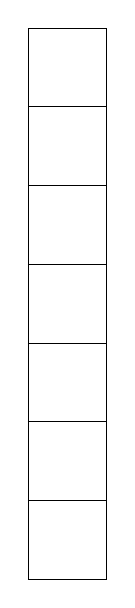
\begin{tikzpicture}
		\draw[step=1cm,black,very thin] (8,-0) grid (9,7);
	\end{tikzpicture}}
\end{minipage}
\def\rowperm{{0, 1, 2, 3, 4, 5, 6}}
%\def\colperm{{0, 1, 2, 3, 4, 5, 6}}
\def\colperm{{0, 1, 2, 3, 4, 5, 6}}
\begin{minipage}{0.55\textwidth}
\centering
\scalebox{0.7}{\begin{tikzpicture}
	\foreach \x in {0,1}
	\fill[red] (\colperm[\x]-1,6) rectangle (\colperm[\x],7);  
	\foreach \x in {0,1,2}
	\fill[red] (\colperm[2+\x]-1,5) rectangle (\colperm[2+\x],6);   
	\foreach \x in {0,1}
	\fill[red] (\colperm[5+\x]-1,4) rectangle (\colperm[5+\x],5); 

	\node at (\colperm[0]-0.5,6.5) {\Large{1}}; 
	\node at (\colperm[1]-0.5,6.5) {\Large{1}}; 
	
	\node at (\colperm[2]-0.5,5.5) {\Large{2}}; 
	\node at (\colperm[3]-0.5,5.5) {\Large{2}}; 
	\node at (\colperm[4]-0.5,5.5) {\Large{2}}; 
	
	\node at (\colperm[5]-0.5,4.5) {\Large{3}}; 
	\node at (\colperm[6]-0.5,4.5) {\Large{3}}; 
	
	\draw[step=1cm,black,very thin] (-1,-0) grid (6,7);
\end{tikzpicture}}
\hspace{0.3cm}
\scalebox{0.7}{\begin{tikzpicture}
	\foreach \x in {0,1,2,3,4,5,6}
	\fill[red] (8,\x) rectangle (9,\x+1);  
	\draw[step=1cm,black,very thin] (8,-0) grid (9,7);
	\node at (8.5,6.5-\colperm[0]) {\Large{1}}; 
	\node at (8.5,6.5-\colperm[1]) {\Large{1}}; 
	\node at (8.5,6.5-\colperm[2]) {\Large{2}}; 
	\node at (8.5,6.5-\colperm[3]) {\Large{2}}; 
	\node at (8.5,6.5-\colperm[4]) {\Large{2}}; 
	\node at (8.5,6.5-\colperm[5]) {\Large{3}}; 
	\node at (8.5,6.5-\colperm[6]) {\Large{3}}; 
\end{tikzpicture}}
\end{minipage}
\begin{minipage}{0.55\textwidth}
	\centering
	\scalebox{0.7}{\begin{tikzpicture}

	\foreach \x in {0,1,2}
	\fill[green] (\colperm[\x]-1,3) rectangle (\colperm[\x],4);  
	\foreach \x in {0,1,2}
	\fill[green] (\colperm[3+\x]-1,2) rectangle (\colperm[3+\x],3);   
	\draw[step=1cm,gray,very thin] (-1,-0) grid (6,7);

	\node at (\colperm[0]-0.5,3.5) {\Large{1}}; 
	\node at (\colperm[1]-0.5,3.5) {\Large{1}}; 
	\node at (\colperm[2]-0.5,3.5) {\Large{1}}; 
	\node at (\colperm[3]-0.5,2.5) {\Large{2}}; 
	\node at (\colperm[4]-0.5,2.5) {\Large{2}}; 
	\node at (\colperm[5]-0.5,2.5) {\Large{2}}; 
	\end{tikzpicture}}
	\hspace{0.3cm}
	\scalebox{0.7}{\begin{tikzpicture}
		\foreach \x in {0,1,2,3,4,5}
		\fill[green] (8,6-\colperm[\x]) rectangle (9,6-\colperm[\x]+1);  
		\draw[step=1cm,gray,very thin] (8,-0) grid (9,7);
		\node at (8.5,6.5-\colperm[0]) {\Large{1}}; 
		\node at (8.5,6.5-\colperm[1]) {\Large{1}}; 
		\node at (8.5,6.5-\colperm[2]) {\Large{1}}; 
		\node at (8.5,6.5-\colperm[3]) {\Large{2}}; 
		\node at (8.5,6.5-\colperm[4]) {\Large{2}}; 
		\node at (8.5,6.5-\colperm[5]) {\Large{2}}; 
		\end{tikzpicture}}
\end{minipage}
\begin{minipage}{0.55\textwidth}
	\centering
	\scalebox{0.7}{\begin{tikzpicture}	
		\foreach \x in {0,1,2}
		\fill[blue] (\colperm[1+\x]-1,1) rectangle (\colperm[1+\x],2);  
		\foreach \x in {0,1,2}
		\fill[blue] (\colperm[4+\x]-1,0) rectangle (\colperm[4+\x],1);
		\draw[step=1cm,gray,very thin] (-1,-0) grid (6,7);   
	
		\node at (\colperm[1]-0.5,1.5) {\Large{1}}; 
		\node at (\colperm[2]-0.5,1.5) {\Large{1}}; 
		\node at (\colperm[3]-0.5,1.5) {\Large{1}}; 
		\node at (\colperm[4]-0.5,0.5) {\Large{2}}; 
		\node at (\colperm[5]-0.5,0.5) {\Large{2}}; 
		\node at (\colperm[6]-0.5,0.5) {\Large{2}}; 
		\end{tikzpicture}}
	\hspace{0.3cm}
	\scalebox{0.7}{\begin{tikzpicture}
		\foreach \x in {0,1,2,3,4,5}
		\fill[blue] (8,\x) rectangle (9,\x+1);  
		\draw[step=1cm,gray,very thin] (8,-0) grid (9,7);
		\node at (8.5,6.5-\colperm[1]) {\Large{1}}; 
		\node at (8.5,6.5-\colperm[2]) {\Large{1}}; 
		\node at (8.5,6.5-\colperm[3]) {\Large{1}}; 
		\node at (8.5,6.5-\colperm[4]) {\Large{2}}; 
		\node at (8.5,6.5-\colperm[5]) {\Large{2}}; 
		\node at (8.5,6.5-\colperm[6]) {\Large{2}}; 
		\end{tikzpicture}}
\end{minipage}
\end{document}
